\documentclass[11pt]{article}
\usepackage{enumerate}
\usepackage[utf8]{inputenc}
\usepackage{fullpage}
\usepackage{amsmath}
\usepackage{amssymb}
\usepackage{graphicx}
\usepackage{float}
\usepackage{listings}
\usepackage{xcolor}
\usepackage{pdfpages}
\usepackage{caption}
\usepackage{subcaption}
\usepackage{lastpage}
%\usepackage[norsk]{babel}

\newenvironment{bottompar}{\par\vspace*{\fill}}{\clearpage}

\DeclareFixedFont{\ttb}{T1}{txtt}{bx}{n}{8} % for bold
\DeclareFixedFont{\ttm}{T1}{txtt}{m}{n}{8}  % for normal

\definecolor{codegreen}{rgb}{0,0.6,0}
\definecolor{codegray}{rgb}{0.5,0.5,0.5}
\definecolor{codepurple}{rgb}{0.58,0,0.82}
\definecolor{backcolour}{rgb}{0.95,0.95,0.92}
 
\lstdefinestyle{mystyle}{
    backgroundcolor=\color{backcolour},   
    commentstyle=\color{codegreen},
    keywordstyle=\color{magenta},
    numberstyle=\tiny\color{codegray},
    stringstyle=\color{codepurple},
    basicstyle=\ttfamily\small,
    breakatwhitespace=false,         
    breaklines=true,                 
    captionpos=b,                    
    keepspaces=true,                 
    numbers=left,                    
    numbersep=3pt,                  
    showspaces=false,                
    showstringspaces=false,
    showtabs=false,                  
    tabsize=3
}
 
\lstset{style=mystyle}

\newcounter{excount}
\newenvironment{exercise}[1][]{\addtocounter{excount}{1} \noindent {\bf Exercise
    \arabic{excount} #1}\hspace{2mm}}{\vspace{4mm}}

\renewcommand{\d}{\mathrm{d}}
%%%%%%%%%%%%%%%%%%%%%%%%%%%%%%%%%%%%%
\newcommand{\ObligNumber}{5 }
%%%%%%%%%%%%%%%%%%%%%%%%%%%%%%%%%%%%%
\begin{document}
\title{\begin{huge}FYS2160 ---  Oblig \ObligNumber\end{huge}}
\author{Ole Gunnar Johansen}

\maketitle
\noindent

\begin{center}
 \textbf{I would like feedback on this oblig.\\}
\end{center}
\begin{exercise}
	\begin{itemize}
		\item[a)]
			The partition function is defined by
			\begin{align*}
				Z = \sum_{\mathrm{All \ states} \ i} e^{-\varepsilon_i/kT}
			\end{align*}
			where $\varepsilon_i$ is the energy of the state $i$.
			
			We are now looking at one particle with motion described by the states $n_x = 0,1,2,...$, and the energy of state $n_x$ is $\varepsilon(n_x) = an_x^2$, where $a=h^2/(8mL^2)$. The partition function for this particle is then
			\begin{align*}
				Z_{1,x} = \sum_{n_x=0}^\infty e^{-an_x^2/kT}
			\end{align*}
			As discussed on the previous week's project, in the high-temperature limit, the above expression can be approximated by an integral (see figure~\ref{fig: illustration of sum to integral task a}). This leads us to
			\begin{align}
				Z_{1,x} 									&\approx \int_{0}^{\infty} e^{-an_x^2/kT} \ dn_x  \nonumber \\
				\lambda^2 \equiv a/kT \rightarrow	&= \int_{0}^{\infty} e^{-\lambda^2n_x^2} \ dn_x \nonumber \\
																&= \frac{\sqrt{\pi}}{2\lambda} \nonumber \\
																&= \frac{1}{2}\sqrt{\frac{kT\pi}{h^2}8mL^2} \nonumber \\
																&= \sqrt{\frac{2\pi mkT}{h^2}}L \label{eq: part.func one part. 1D evaluated}
			\end{align}
			where I used the solution to the integral given in the exercise:
			\begin{align*}
				\int_{0}^{\infty} e^{-\lambda^2x^2} \ dx = \frac{\sqrt{\pi}}{2\lambda}
			\end{align*}
			
			\begin{figure}
				\centering
				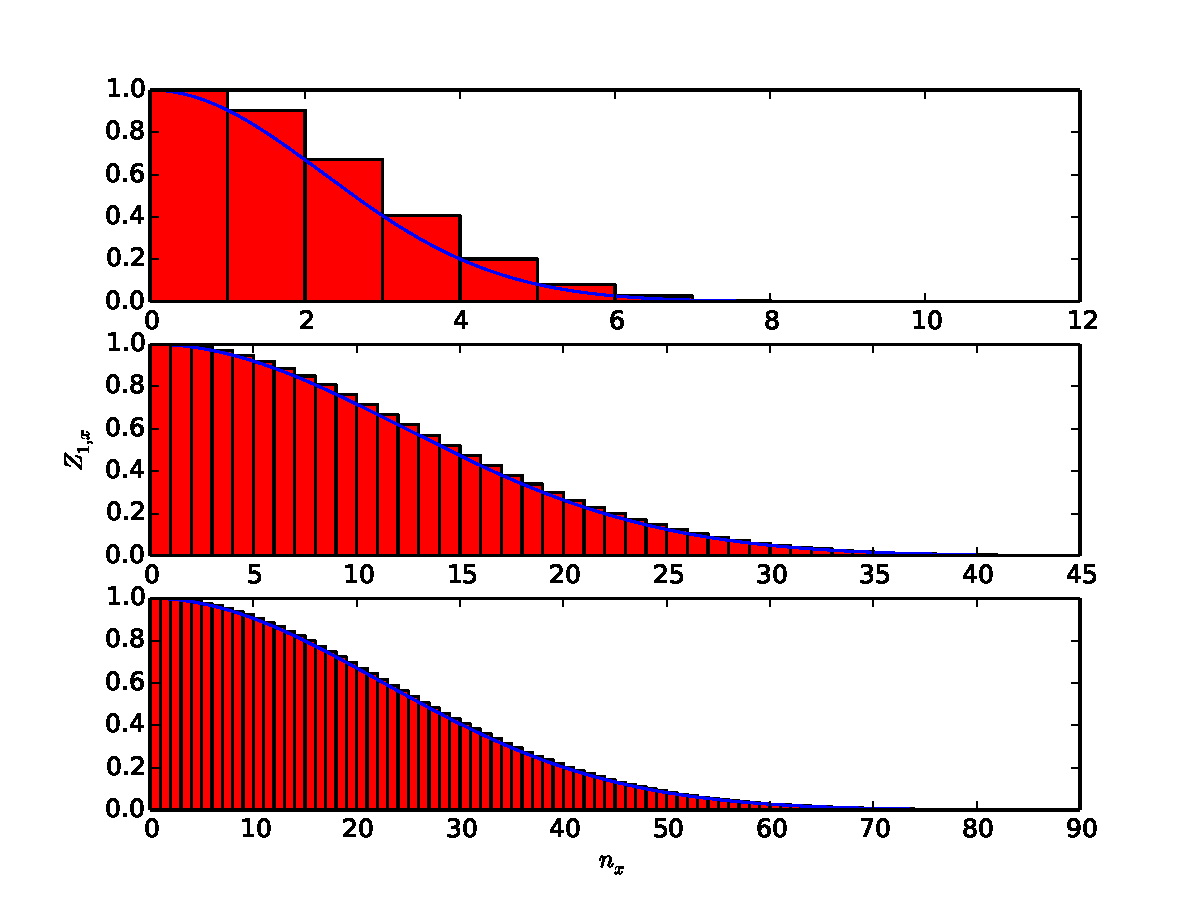
\includegraphics[scale=0.7, clip=true, trim= 0 0 0 0]{task_a_illustration.pdf}
				\caption{Illustration that the partition function becomes more and more equal an integral for high temperatures. The figure shows three plots with the terms in the partition function plotted on the $x$-axis and for increasing temperatures down (top is lowest temperature, bottom is highest).}
				\label{fig: illustration of sum to integral task a}
			\end{figure}
			
			
			
			
		\item[b)]
			For $2$ particles moving in one direction, the partition function would read
			\begin{align*}
				Z_{2,x} 	&= \sum_{n_{x_1}=0}^\infty \sum_{n_{x_2}=0}^\infty e^{-[\varepsilon(n_{x_1}) + \varepsilon(n_{x_2})]/kT} \\
								&= \sum_{n_{x_1}=0}^\infty \sum_{n_{x_2}=0}^\infty e^{-\varepsilon(n_{x_1})/kT}e^{-\varepsilon(n_{x_2})/kT} \\
								&=  \sum_{n_{x_1}=0}^\infty e^{-\varepsilon(n_{x_1})/kT}\sum_{n_{x_2}=0}^\infty e^{-\varepsilon(n_{x_2})/kT} \\
								&= Z_{1,x}^2
			\end{align*}
			In the general case, we get
			\begin{align*}
				Z_{N,x} = Z_{1,x}^N
			\end{align*}
			Note, however, that this is for a gas which is made up of distinguishable particles. The ideal gas in question, can, however, be assumed to be made up of indistinguishable particles, meaning we can swap any two particles in different states and still have the same gas. Some particle states have therefore been counted twice, resulting in\footnote{Following the derivation in section 6.6 of Schroeder's book on thermal physics (2000), we ignore the fact that interchanging to particles with the same states, have not, in fact, been counted twice. This is an approximation which, to a great extent, is valid for low density gases.}
			\begin{align}
				Z_{N,x} = \frac{1}{N!}Z_{1,x}^N = \frac{1}{N!}\left( \frac{2\pi mkT}{h^2} \right) ^{N/2}L^N \label{eq: part func 1D gas N particles}
			\end{align}
		
		
		\item[c)]
			The total average energy of the gas is
			\begin{align*}
				U = -\frac{1}{Z}\frac{\partial Z}{\partial \beta}
			\end{align*}
			where $\beta = 1/(kT)$. Using the partition function in eq.~\eqref{eq: part func 1D gas N particles}, we get
			\begin{align*}
				U 	&= -\left[ \frac{1}{N!}\left( \frac{2\pi m}{\beta h^2} \right) ^{N/2}L^N \right]^{-1}\frac{\partial}{\partial \beta} \left[ \frac{1}{N!}\left( \frac{2\pi m}{\beta h^2} \right) ^{N/2}L^N \right] \\
					&= -\left[ \frac{1}{N!}\left( \frac{2\pi m}{\beta h^2} \right) ^{N/2}L^N \right]^{-1} \left[\frac{1}{N!}\left( \frac{2\pi m}{h^2} \right) ^{N/2}L^N \right] \frac{\partial}{\partial \beta} \beta ^{-N/2} \\
					&= -\beta^{N/2}\left( -\frac{N}{2} \right) \beta^{-N/2 - 1} \\
					&= \frac{N}{2\beta} = \frac{1}{2}NkT
			\end{align*}
		
		
		\item[d)]
			% see page 255 and 11.3
			For the canonical system, we found the quantity called Helmholtz free energy: $F=E-TS$. Where $F$ can be calculated by
			\begin{align*}
				F = -kT\ln Z
			\end{align*}
			Taking the differential of $F$ we obtain
			\begin{align*}
				dF 	&= dE - SdT - TdS \\
						&= dE - SdT - dE - PdV + \mu dN \\
						\Rightarrow S &= -\left( \frac{\partial F}{\partial T} \right) _{V,N}
			\end{align*}
			So, all we need to do is calculate $F_{N,x}$:
			\begin{align*}
				F_{N,x}	&= -kT\ln Z_{N,x} \\
							&= -kT \ln \left[ \frac{1}{N!}\left( \frac{2\pi mkT}{h^2} \right) ^{N/2} L^N \right] \\
							&= -kT \left[ -\ln N! + \frac{N}{2}\ln \left( \frac{2\pi mkT}{h^2} \right) + N\ln L  \right]
			\end{align*}
			and so, the entropy is
			\begin{align*}
				S 	&= -\frac{\partial}{\partial T} \left[ kT \left[ \ln N! - \frac{N}{2}\ln \left( \frac{2\pi mkT}{h^2} \right) - N\ln L  \right] \right]_{N,V} \\
					&=  -k\ln N! + \frac{Nk}{2}\ln \left( \frac{2\pi mkT}{h^2} \right) + \frac{NkT}{2} \frac{h^2}{2\pi mkT} \frac{2\pi mk}{h^2} \\
					&= -k\ln N! + \frac{Nk}{2}\ln \left( \frac{2\pi mkT}{h^2} \right) + \frac{Nk}{2}
			\end{align*}
		
		
		
		
		\item[e)]
			Opening for the possibility that the particles can move freely in 2 dimensions, the energy associated with each particle is
			\begin{align*}
				\varepsilon(n_x, n_y) = an_x^2 + an_y^2
			\end{align*}
			The partition function for one particle then reads
			\begin{align*}
				Z_{1,x,y} 	&= \sum_{n_x=0}^{\infty} \sum_{n_y=0}^\infty e^{-an_x^2/kT}e^{-an_y^2/kT} \\
								&= \sum_{n_x=0}^{\infty}  e^{-an_x^2/kT} \sum_{n_y=0}^\infty e^{-an_y^2/kT}
			\end{align*}
			We recognize that the first sum in the above expression is the same as for one particle moving in one dimension, which can be evaluated as in eq.~\ref{eq: part.func one part. 1D evaluated}. We also recognize that the second sum above has the same value as the first, leading to the partition function being:
			\begin{align}
				Z_{1,x,y} = Z_{1,x}^2 \label{eq: part.func. 2D one particle}
			\end{align}
			
			Following the same set of steps as in ex. b), we find that for $N$ particles, the partition function is
			\begin{align}
				Z_{N,x,y} = Z_{1,x}^{2N} \label{eq: part.func. 2D}
			\end{align}
			which in turn implies that the total average energy of the ideal gas is
			\begin{align}
				U = -\frac{1}{Z}\frac{\partial Z_{n,x,y}}{\partial \beta}  = \cdots = NkT \nonumber
			\end{align}
			and the entropy is
			\begin{align}
				S &= -\left( \frac{\partial F}{\partial T} \right) _{V,N} \nonumber \\
				\cdots &= -k\ln N! + Nk + Nk\ln \left( \frac{2\pi mkT}{h^2} \right) - 2Nk\ln L \nonumber
			\end{align}
			where Helmholtz free energy is
			\begin{align}
				F = -kT \left[-\ln N! + N\ln \left( \frac{2\pi mkT}{h^2} \right) + 2N\ln L \right] \nonumber
			\end{align}
		
		\item[f)]
			 The energy of this system is
			 \begin{align}
			 	\varepsilon_{3D} = an_x^2 + an_y^2 + \varepsilon_{z0} \nonumber
			 \end{align}
			 So the partition function is
			 \begin{align}
			 	Z_{1,3D} 	&= \sum_{\mathrm{all~states}} e^{-\varepsilon_{3D}/kT} \nonumber \\
			 		&= \sum_{n_x=0}^\infty \sum_{n_y=0}^{\infty} e^{-an_x^2/kT}e^{-an_y^2/kT}e^{-\varepsilon_{z0}/kT} \nonumber \\
			 		&= \sum_{n_x=0}^\infty e^{-an_x^2/kT} \sum_{n_y=0}^{\infty} e^{-an_y^2/kT} e^{-\varepsilon_{z0}/kT} \nonumber \\
			 		&= Z_{1,2D} e^{-\varepsilon_{z0}\beta} \nonumber
			 \end{align}
			 where $Z_{1,2D}$ is the partition function for one particle the two dimensional case in eq.~\ref{eq: part.func. 2D one particle} and $\varepsilon_{z0}$ is the energy for the ground state for for motion in the $z$-direction.
			 For $N$ particles:
			 \begin{align}
			 	Z 	&= \frac{1}{N!}Z_{1,3D}^N \nonumber \\
			 		&= \frac{1}{N!}Z_{1,2D}^N e^{-N\varepsilon_{z0}\beta} \nonumber \\
			 		&= Z_{N,2D} e^{-N\varepsilon_{z0}\beta} \nonumber
			 \end{align}
			 where again, $Z_{N,2D}$ is the partition function for $N$ particles in the two dimensional case in eq.~\ref{eq: part.func. 2D}. 
			
		
		\item[g)]
			Using the above expression for the partition function in three dimensions, the energy can be calculated as
			\begin{align}
				U 	&= -\frac{1}{Z}\frac{\partial Z}{\partial \beta} \nonumber \\
					&= -\frac{1}{Z}\frac{\partial}{\partial \beta} \left( Z_{N,2D} e^{-N\varepsilon_{z0}\beta} \right) \nonumber \\
					&= -\frac{1}{Z}\left[ e^{-N\varepsilon_{z0}\beta} \frac{\partial}{\partial \beta} Z_{N,2D} + Z_{N,2D}\frac{\partial}{\partial \beta}e^{-N\varepsilon_{z0}\beta} \right] \nonumber \\
					&= -\frac{1}{Z} \left[ e^{-N\varepsilon_{z0}\beta} \left( -U_{2D} Z_{N,2D} \right) - Z_{N,2D} N \varepsilon_{z0} e^{-N\varepsilon_{z0}\beta} \right] \nonumber \\
					&= -\frac{1}{Z_{N,2D} e^{-N\varepsilon_{z0}\beta}} Z_{N,2D} e^{-N\varepsilon_{z0}\beta} \left( -N \varepsilon_{z0} -U_{2D} \right) \nonumber \\
					&= U_{2D} +  N \varepsilon_{z0} \nonumber  \\
					&= NkT + N \varepsilon_{z0} \nonumber
			\end{align}
			
			
			
	\end{itemize}
\end{exercise}


\begin{exercise}
	\begin{itemize}
		\item[a)]
			The gas is taken into the engine before 1 in the figure. In a single cycle, the gas is first compressed adiabatically from $1\rightarrow 2$, implying no change in entropy. The same applies for the processes in $3\rightarrow 4$. In $2\rightarrow 3$ and $4\rightarrow 1$, however, the processes are not adiabatic, so the entropy changes. The question is, then, by how much?

			The PV-diagram shows the gas which is in the chamber at all times. Since processes are assumed to be reversible, it doesn't matter if we start to study the cycle after 1 cycle or 20 000 cycles. The entropy of the system must therefore be the same at 1, no matter where we start looking at it, and so $\Delta S_{23} = -\Delta S_{41}$, and for the whole cycle $\Delta S = \Delta S_{23} + \Delta S_{41} = 0$.			
		
		
		\item[b)]
			The entropy of an ideal gas is given by the Sackur-Tetrode equation:
			\begin{align*}
				S = Nk\left[ \ln \left( \frac{V_2}{N} \left( \frac{4\pi mk T}{h^2} \right) ^{3/2} \right) + \frac{5}{2} \right]
			\end{align*}
			The change in entropy between the initial state $s_i=s(V_i, T_i)$ and the final state $s_f=s(V_f, T_f)$ is then
			\begin{align}
				\Delta S_{s_i s_f} = S_{s_f} - S_{s_i} = Nk\ln \left( \frac{V_f T_f^{3/2}}{V_i T_i^{3/2}} \right) \label{delta S si sf}
			\end{align}
			Using that in $2\rightarrow 3$, the pressure in the gas, can be written as
			\begin{align*}
				\frac{NkT_2}{V_2} = P_2 = P_3 = \frac{NkT_3}{V_3}
			\end{align*}
			we find that the change in entropy is
			\begin{align*}
				\Delta S_{23} = Nk\ln \left( \frac{V_3 T_3^{3/2}}{V_2T_2^{3/2}} \right) = Nk\ln \left( \frac{T_3V_2 T_3^{3/2}}{T_2 T_2^{3/2}} \right)  = \frac{5}{2}Nk\ln\frac{T_3}{T_2} = C_P\ln \frac{T_3}{T_2}
			\end{align*}
			where $C_P = \frac{5}{2}Nk$.
		
		\item[c)]
			Since there is no work done on the system for the case $4\rightarrow 1$, we can use the definition of heat capacity of constant volume:
			\begin{align}
				C_V = \frac{\partial Q}{\partial T} \Rightarrow dQ = C_V dT \label{eq: heat capacity constant volume}
			\end{align}
			and the definition of temperature to calculate the change in entropy. The definition of temperature is
			\begin{align*}
				ds = \frac{dQ}{T} \Rightarrow \Delta S_{T_i, T_f} &= \int_{T_i}^{T_f} \frac{dQ}{T} = C_V \int_{T_i}^{T_f} \frac{dT}{T} \\
				\Rightarrow \Delta S_{41} = C_V \int_{T_4}^{T_1} \frac{dT}{T} = C_V \ln \frac{T_1}{T_4}
			\end{align*}
		
		
		\item[d)]
			Using the above expressions for $\Delta S_{23}$ and $\Delta S_{41}$:
			\begin{align*}
				\frac{\Delta S_{23}}{\Delta S_{41}} &= \frac{C_P}{C_V}\frac{\ln(T_3/T_2)}{\ln(T_1/T_4)} \\
				\Rightarrow \left( \frac{T_1}{T_4} \right)^{\frac{\Delta S_{23}}{\Delta S_{41}}} &= \left( \frac{T_3}{T_2} \right) ^\gamma \\
				\Rightarrow T_1^\frac{\Delta S_{23}}{\Delta S_{41}}T_2^\gamma &= T_3^\gamma T_4^\frac{\Delta S_{23}}{\Delta S_{41}}
			\end{align*}
			where $\gamma = C_P/C_V$. Using the result from a), we find that $\frac{\Delta S_{23}}{\Delta S_{41}}=-1$ and the above expression is the desired one.
		
		
		\item[e)]
			The average thermal energy of the ideal gas is $Q=\frac{3}{2}NkT$. This is at constant volume. Following the definition of heat capacity, the heat capacity at constant volume is the temperature derivative of the thermal energy, and so $C_V = \frac{3}{2}Nk$, or
			\begin{align*}
				\gamma = \frac{C_P}{C_V} = \frac{5}{3}
			\end{align*}
			
			Using eq.~\eqref{delta S si sf}, we then find that the change in entropy between state 1 and state 2 is
			\begin{align*}
				\Delta S_{12} = Nk\ln \left( \frac{V_2T_2^{3/2}}{V_1T_1^{3/2}} \right)
			\end{align*}
			Since the process is adiabatic, $\Delta S_{12} = 0$, and so we find
			\begin{align*}
				V_1T_1^{3/2} = V_2T_2^{3/2} \Rightarrow V_1^{2/3}T_1 &= V_2^{2/3}T_2 \\
				V_1^{\gamma-1}T_1 &= V_2^{\gamma-1}T_2
			\end{align*}
			And very similar for the process $3\rightarrow 4$, we find
			\begin{align*}
				V_3^{\gamma - 1}T_3 = V_1^{\gamma-1}T_4
			\end{align*}
			
		
		\item[f)]
			Using eq.~\eqref{eq: heat capacity constant volume} we find that 
			\begin{align*}
				Q_{41} = C_V\int_{T_4}^{T_1} dT = C_V(T_1 - T_4)
			\end{align*}
			The definition of heat capacity of constant pressure is exactly equal to that in eq.~\eqref{eq: heat capacity constant volume}, so we get, again
			\begin{align*}
				Q_{23} = C_P \int_{T_2}^{T_3} dT = C_P(T_3-T_2)
			\end{align*}
		
		\item[g)]
			The ideal efficiency is 
			\begin{align*}
				e = 1 - \frac{Q_{\mathrm{in}}}{Q_{\mathrm{out}}}
			\end{align*}
			where, in this case, heat is added when the fuel is ignited in $2\rightarrow 3$ and heat is taken out in $4\rightarrow 1$. Therefore, the ideal efficiency is
			\begin{align*}
				e = 1-\frac{-C_V(T_1 - T_4)}{C_P(T_3-T_2)} = 1-\frac{C_V(T_4 - T_1)}{C_P(T_3-T_2)}
			\end{align*}
			
			
	\end{itemize}
\end{exercise}


\begin{bottompar}
\begin{center}
	End of oblig \ObligNumber
\end{center}
\end{bottompar}
\end{document}